\documentclass[11pt,a4paper]{article}
\usepackage[utf8]{inputenc}
\usepackage[T1]{fontenc}
\usepackage[margin=1in]{geometry}
\usepackage{graphicx}	
\usepackage{hyperref}
\usepackage{xcolor}

\hypersetup{
    colorlinks=true,
    linkcolor=blue,			
    filecolor=magenta,      
    urlcolor=blue,
    hidelinks,
    %pdftitle={The Financial Benefits of Accessible Digital Design}
}

\graphicspath{{Web_accessibility_images/}} % add changes 15.11.2026

%%%%%%%%%%%%%%%%%%%%%%%%%%%%%%%%%% HEAD OF DOCUMENT

\title{Web Accessibility Documentation}											
\author{Shalini Denti, Manuel Pollazzon, Andrii Synelnyk}
\date{08.11.2026}

%%%%%%%%%%%%%%%%%%%%%%%%%%%%%%%%%% FRONT PAGE + TABLE OF CONTENTS [COMPLETE]

\begin{document}
\maketitle

\pagecolor{white}
\tableofcontents

\newpage

%%%%%%%%%%%%%%%%%%%%%%%%%%%%%%%%%% PART 1 [COMPLETE] ~ Pollazzon

\section{WCAG Guidelines and Standards}

	\subsection{Part 1: Web Accessibility Principles (The POUR Framework)}

	WCAG 2.2 is organized around four foundational principles ---
	\emph{Perceivable, Operable, Understandable, Robust} --- each of which
	subsumes a set of normative guidelines.

		\subsubsection{Principle 1 --- Perceivable} 
		
		Information and user interface components must be presentable to users in ways
		they can perceive.

		\begin{itemize}
		  \item \textbf{1.1 Text Alternatives} --- Provide text alternatives for any
       		 non-text content.
 		 \item \textbf{1.2 Time-based Media} --- Provide alternatives for time-based
        		media (captions, audio description).
		  \item \textbf{1.3 Adaptable} --- Create content that can be presented in
       		 different ways without losing structure.
  		\item \textbf{1.4 Distinguishable} --- Make it easier to see and hear
      		  content, including separating foreground from background.
		\end{itemize}


		\subsubsection{Principle 2 --- Operable}
		User interface components and navigation must be operable.
		
		\begin{itemize}
 		 \item \textbf{2.1 Keyboard Accessible} --- Make all functionality available
      		  from a keyboard.
		  \item \textbf{2.2 Enough Time} --- Provide users enough time to read and use
       		 content.
 		 \item \textbf{2.3 Seizures and Physical Reactions} --- Do not design content
    		    in a way that is known to cause seizures.
		  \item \textbf{2.4 Navigable} --- Provide ways to help users navigate, find
    		    content, and determine where they are.
		  \item \textbf{2.5 Input Modalities} --- Make it easier to operate
       		 functionality through various inputs beyond the keyboard.
		\end{itemize}

		
		\subsubsection{Principle 3 --- Understandable}
		Information and the operation of the user interface must be understandable.
		\begin{itemize}
		  \item \textbf{3.1 Readable} --- Make text content readable and
       		 understandable.
		  \item \textbf{3.2 Predictable} --- Make web pages appear and operate in
       		 predictable ways.
		  \item \textbf{3.3 Input Assistance} --- Help users avoid and correct
      		  mistakes.
		\end{itemize}


		\subsubsection{Principle 4 --- Robust}
		Content must be robust enough that it can be interpreted reliably by a wide
		variety of user agents, including assistive technologies.
		
		\begin{itemize}
 		 \item \textbf{4.1 Compatible} --- Maximize compatibility with current and
     		   future user agents (note: \emph{4.1.1 Parsing} was removed in WCAG
     		   2.2).
		\end{itemize}


	\subsection{Part 2: Compliance Levels and Conformance Framework}

		\subsubsection{The Three Conformance Levels}
		Every success criterion in WCAG 2.2 is assigned one of three levels:

		\begin{itemize}
		  \item \textbf{Level A} --- Minimum baseline. Non-negotiable for any
     		   accessible system.
		  \item \textbf{Level AA} --- Standard target for most legal and procurement
   		     frameworks (e.g., EU EN 301 549, US Section 508, ADA-aligned policy).
		  \item \textbf{Level AAA} --- Enhanced, contextual conformance; not
     		   recommended as a blanket site-wide target.
		\end{itemize}


		\subsubsection{The Five Conformance Requirements}
		WCAG 2.2 defines five conformance requirements:
	
		\begin{enumerate}
 		 \item \textbf{Conformance Level} --- Fully satisfy all requirements of the
    		    chosen level.
		  \item \textbf{Full Pages} --- Conformance applies to full web pages, not
    		    fragments.
		  \item \textbf{Complete Processes} --- Every step in a multi-step process must
  		      conform.
		  \item \textbf{Only Accessibility-Supported Ways} --- Use only
    		    accessibility-supported technologies.
		  \item \textbf{Non-Interference} --- No content may interfere with the
        accessibility of other content.
		\end{enumerate}

\newpage
%%%%%%%%%%%%%%%%%%%%%%%%%%%%%%%%%% PART 2  [COMPLETE] ~Coffee

\section{Inclusive design principles}

\subsection{Introduction:}
	
	Whether you are a digital designer, a business leader or a product manager, there’s one thing is important in the process: 
	make the product the most accessible for a larger set of costumers. This includes also the way you interact through the interface
	 of a computer to display informations as simple as possible for the costumer in order to get its attention and let him focus on the
	  valuable informations. Not all human are equal in some capacity regarding their senses or the way their mind works. This is the 
	  reason it is needed to accomplish design elements to let the largest amount of people understand what does the screen display 
	  and how to easily interact with it.

	In this section we’re going to first do an overview, to understand where this necessities came from, and then the various 
	subtopics. therefore the subchapter will be
	
	\begin{enumerate}
		\item \textbf{Historical part}
		\item \textbf{Divers users needs}
	\end{enumerate}

	\begin{figure}[h]										
	\centering
			
\includegraphics [width=\textwidth]{./Web_accessibility_images/Accessibility_design_introduction.png}	
			\caption{fig.2.1}
	\end{figure}
	
\subsection{Defining inclusive design in the digital era:}

	As technologies are becoming more and more central in daily life, and the expansion of tech market is enlarging even more, 
	there’s the need to provide to everyone a simple approach of any digital technologies in a digital society.
	It all started back then, when computers were slow machines with low comprehension of inputs of the user with a very complex 
	interface. In a nutshell, the computer accessibility was quite complicated and difficult to understand. As the spectrum of human 
	diversity and capacities deepen, also the design approach evolved too. With the birth of World Wild Web the challenge was set:  
	many web pages had changed styles and tools to be more understandable and approachable for users. By the end of 90’s there was an
	 historical improvement with the publication of \emph{“Web Accessibility guidelines” } where a crucial standard was set and developers 
	 could use a shared framework . Features like keyboard 
	navigation, alternative text for images and other tools that are now the default set of a web page were introduced. All for one goal: make web sites easier.

	Another key accomplishment was reached when web designers shifted from “designing for disabilities” to “design for diversity”.
	Before, designers were designing special features with the only purpose to help disabled people to use interface and other 
	technologies. Even though it was the first and crucial step to help these people, these disability-specific adaptations were 
	targeting
	 disabled people as different. A few times later, designers realized that a bunch of more people could get benefits from some 
	 disability-specific adaptations and conclude that the variants they created could be extended for more people.
	
	\textbf {\emph For example:} Voice control features designed in principle for people with motor disabilities, nowadays they become convenient 
	 for multitasking parents with their hands full; or drivers needing an hand - free operation. So diversity instead of disability.
	 
	 \begin{figure}[h]										
	\centering{
		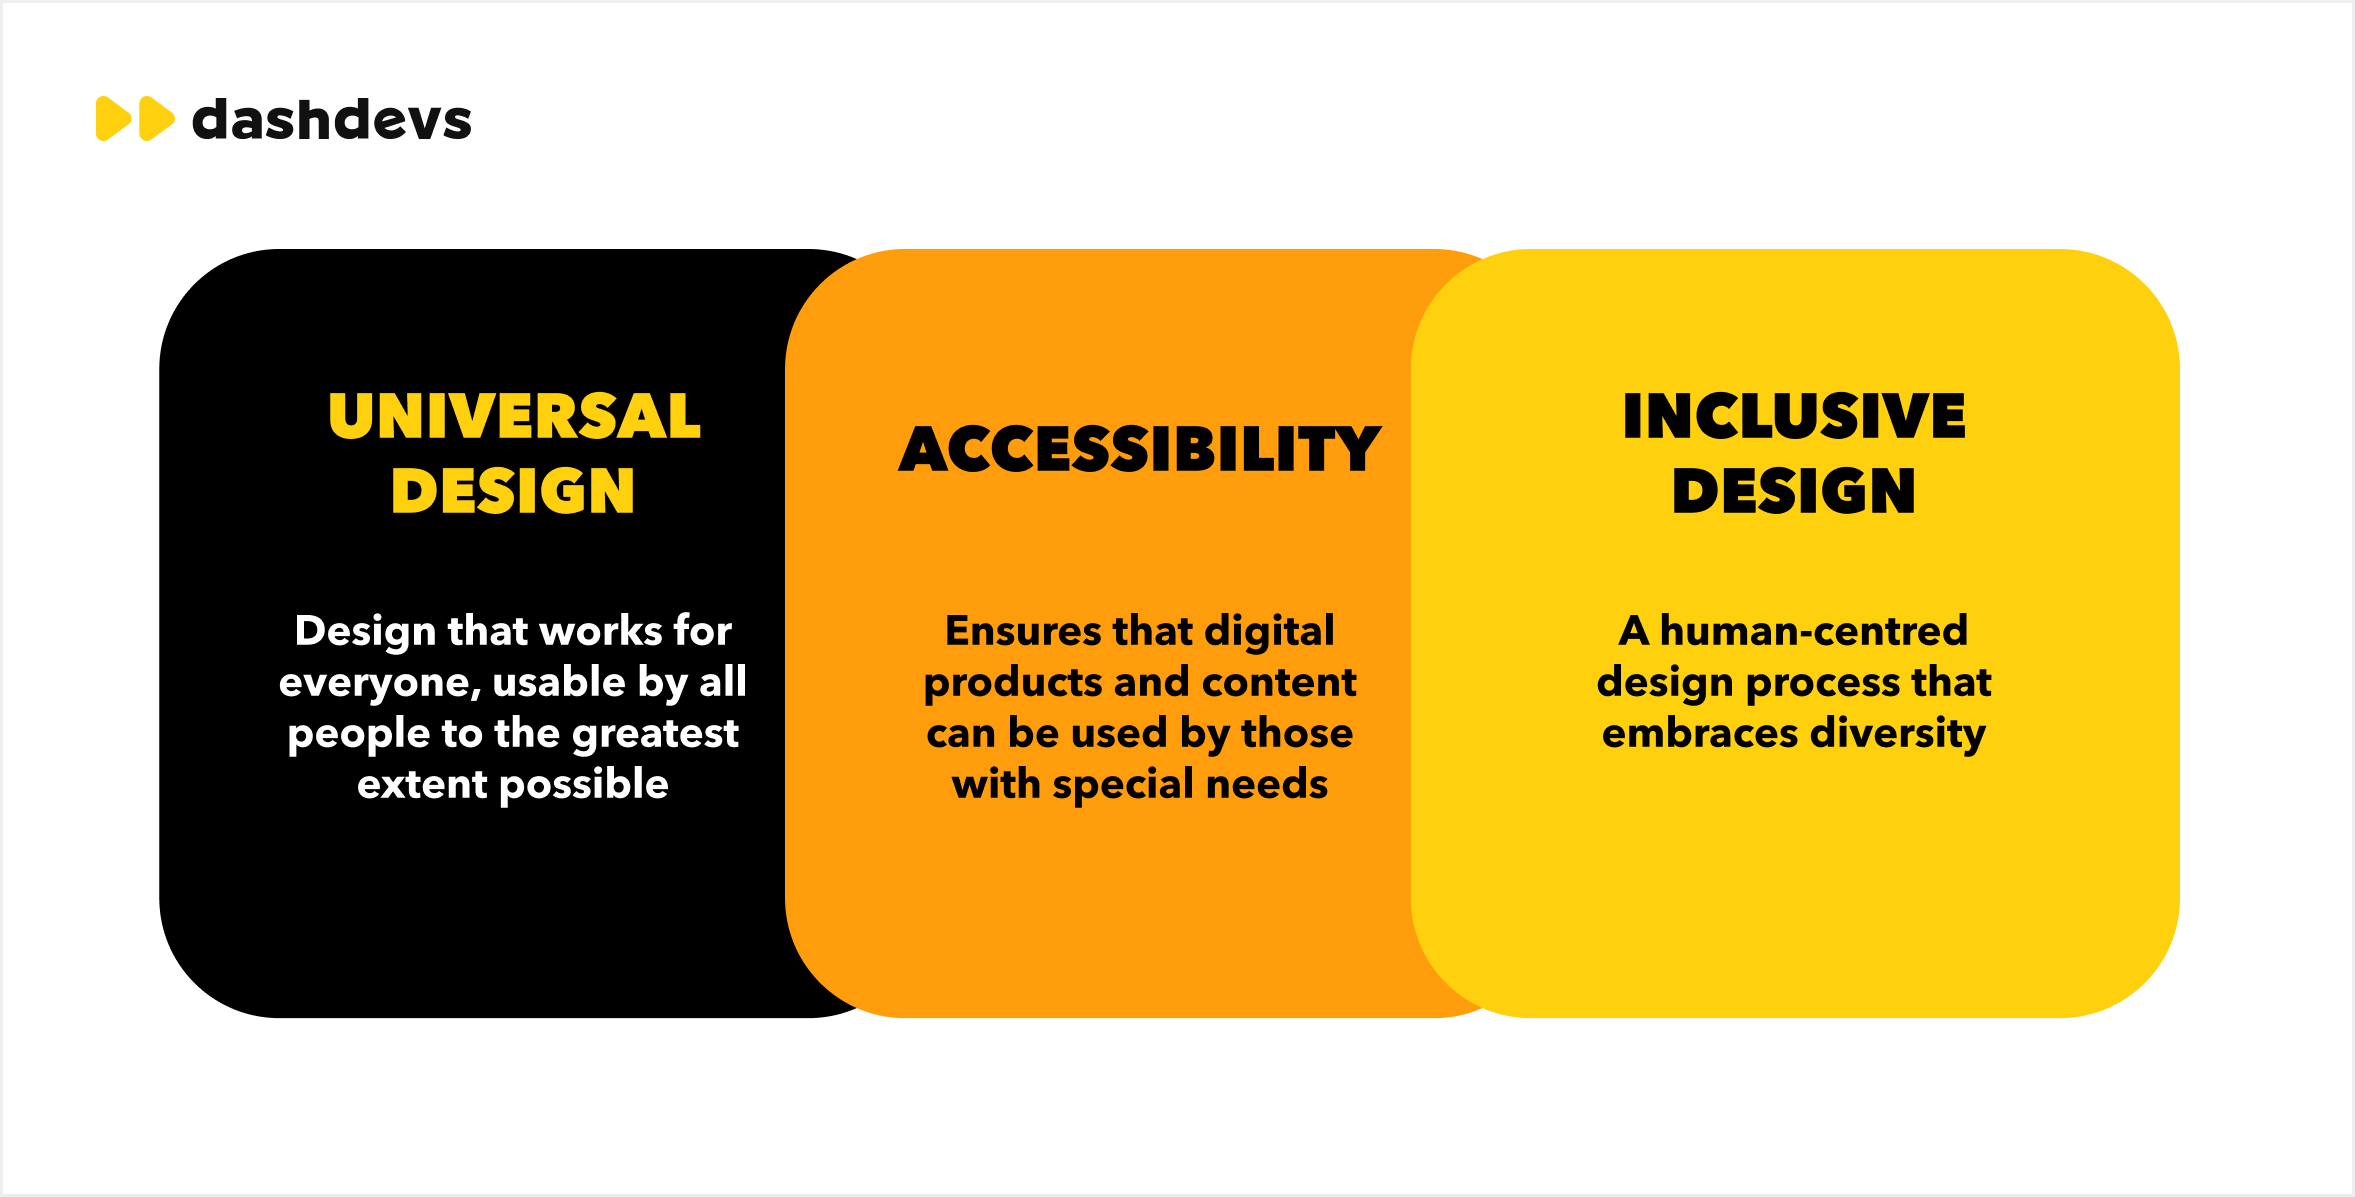
\includegraphics [width=\textwidth]{./Web_accessibility_images/value-adding-benefits-of-mobile-friendly-website-design.jpg}
		\caption{fig.2.2}
	}	
	\end{figure}
	 
	 It is also fair to say that nowadays everyone can have a disability based on the personal condition or the environment they’re in: 
	  a commuter in a bumpy bus, a broken arm, or else; which differs from the historical definition of disability which marked a person as 
	  fundamentally physical different from a normal one. With the new definition a person who cannot do their task properly for any reason, can
	   be "disabled". This is why everyone can benefits from the upgrade of digital system performances: to make everyday challenges smoother.

	In the modern world the disability is not something you are born with until you are in an environment not thought for your needs 
	or your personal shortcomings. This change of mind include a different approach in the code script: it’s not anymore the individual 
	in charge to conform to others but quite the opposite, it’s the society who must conform to itself; hence the web must change for
	 users and users are not required to change or acknowledge things to understand the web. We can say that now the web is more of "full 
	 set of people" oriented and not only for those few smart genius or computer geeks. We can create now a digital space that welcome everyone, 
	 regardless the ability.
	 	  
		 

\subsection{Divers user needs:}

	\textbf{\large Types of disabilities and Assistive technologies:}

	The key of this challenge is first to understand and recognize the divers spectrum of user needs and abilities. In order to 
	acknowledge this concept, we can summarize here the main parameters:
	
	\begin{enumerate}
		\item  \textbf{Types of disabilities:} recognize the duration of disability: temporally, permanent or due to the situation.
		\item \textbf{Accessibility spectrum:} since the accessibilities can be very different and various, the design need to be really 
		flexible to provide solutions for different kind of ability levels. For example adjustable font-size of texts.
		\item \textbf{Intersectionality:} Considering the existence of multiple factors can compound accessibility challenges if some users has more than one shortcomings.
		\item \textbf{Changing needs:} User needs can evolve during time, this put an highlight on elder people who may be limited 
		in mobility and need the web to accommodate their needs.
		\item \textbf{Cultural diversity:} User cultural and linguistic differences can also make improvements in accommodating
		 needs and enlarge the additional tools for people-disabilities orientation. 
	\end{enumerate} 	
	
	\subsubsection*{\textbf{\Large Seven principles of universal design:}}
	It is required a deep knowledge of how different people navigate the digital world.
	Another fundamental concepts are the seven principles of universal design:
	
	\begin{enumerate}
		 \item \textbf{Equitable use:} A website must let everyone decides whether they want to adjust the text size and color contrast 
		 based on their preference.
		 \item \textbf{Flexibility in use:} The website let you decide your kind of interaction with interface: whether you tap, type or talk. 
		 It is better if it includes either fingertips or voice commands.
		\item \textbf{Simple and inductive use:} Simplicity and effectiveness over anything else.
		 \item \textbf{Perceptible information:} A video player offering captions, audio descriptions or else, that ensure you won’t miss
		 any informations.
		\item \textbf{Tolerance for error:}  the website nicely provides to show you your errors without making you feel dumb.
		\item \textbf{Low physical effort:}  implementing shortcuts and content management with bulk actions in order to make every task simpler.
		\item \textbf{Size and space} This translate to design that play nicely with all screens and fingers. Let's create touch targets that are easy to tap and layouts that work great whether you're on a phone or a desktop.
	\end{enumerate}
	 
	 \begin{figure}[h]										
	\centering{
		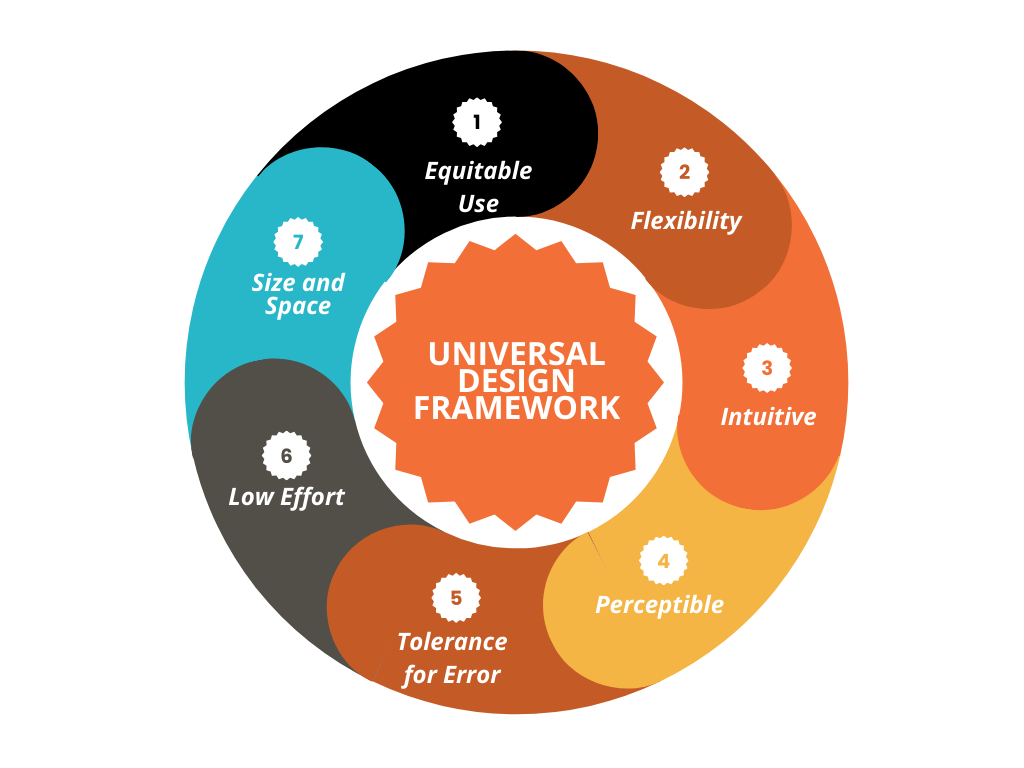
\includegraphics [width=10cm]{./Web_accessibility_images/Universal-Design-Framework.png}
		\caption{2.3}
	}	
	\end{figure}
	
	By prioritizing inclusivity from the beginning, we create digital environments that not only meet diverse needs but also foster innovation
	 and connection of everyone. 
	 Let’s group type of disabilities into categories:
	 
	 \begin{enumerate}
 		\item \textbf{Visual disabilities:} for users who are blind or has a restricted vision it’s essential that an audio form or a more larger size 
		can be fundamentals. Playing also with highlighted words can be really useful and an ordered paragraph can be the key of a 
		better comprehension instead of a chaotic unique paragraph text with no labeling and no images. Alternative methods are 
		implemented to solve this problem as zoom for screen.
		 \item \textbf{Auditory disabilities:} Such as deaf or compromised hearing. It is required alternatives for video or anything that 
		 includes sounds such as transcription of the video. In this case are also used (for example) flashing-lights as Set Alarm to ensure that the 
		 information can reach beyond the limited hearing ability.
		 \item \textbf{Motor disabilities:} can include such as tremors or arthritis to paralysis and amputations. These conditions can affect how
		  people interact with digital devices. A solution can be voice interaction, but for those who also have voice disabilities it 
		  must be implemented other kind of inputs.
		  \item  \textbf{Cognitive disabilities:} for example dyslexia or ADHD, compromise user perception and information can’t be 
		  absorbed. Of course there are many solutions like a more interactive website with many intuitive figures that provide 
		  visual clarity without overstimulating the user.
	\end{enumerate}
	
\newpage
	
%%%%%%%%%%%%%%%%%%%%%%%%%%%%%%%%%% PART 3 [COMPLETE] ~ Pollazzon

\section{Economics of Accessibility}

%% part 3.1 The Financial Benefits of Accessible Digital Design

	\subsection{\Large The Financial Benefits of Accessible Digital Design}

	\subsection{Driving Product Innovation and Usability}
	Designing for edge cases and diverse access needs consistently generates
	mainstream product and technical breakthroughs:
	
	\begin{itemize}
  	\item \textbf{Spillover UX Benefits:} Features initially engineered for
        accessibility---such as voice interaction, auto-complete,
        high-contrast displays, and structured layouts---benefit all users
        operating in glare, high-noise environments, or with limited
        bandwidth.
 	 \item \textbf{Flexible and Responsive Design:} Early compliance with web
        standards accelerated the development of responsive design, ensuring
        seamless performance across varied device form factors.
 	 \item \textbf{Code Quality and Efficiency:} Accessible markup practices
        produce cleaner code structures, reducing long-term technical debt and
        platform maintenance costs.
	\end{itemize}

	\subsection{Expanding Market Reach and Revenue}
	Inclusive design unlocks massive, under-served global demographics:
	
	\begin{itemize}
 	 \item \textbf{Global Spending Power:} Over 1 billion individuals live with
        recognized disabilities, controlling more than \$6 trillion in annual
        disposable income (\$6.9 trillion across the extended network of
        friends and family).
 	 \item \textbf{Regional Demographics:} In the UK, the annual spending power
        of disabled individuals and their families (the ``Purple Pound'')
        exceeds \pounds 249 billion, while US discretionary spending is over
        \$200 billion.
  	\item \textbf{SEO and Discoverability:} Text alternatives such as
        transcripts and semantic headings enhance search engine indexing. For
        instance, NPR's \emph{This American Life} recorded a 6.86\% increase
        in search traffic and a 4.18\% rise in unique visitors after
        publishing text transcripts.
	\end{itemize}

	\subsection{Enhancing Brand Equity and Corporate Reputation}
	A visible commitment to accessibility strengthens Corporate Social
	Responsibility (CSR) initiatives and market positioning:
	\begin{itemize}
 	 \item \textbf{Brand Differentiation:} Proactive accessibility signals
        ethical leadership, enhancing customer retention and brand loyalty
        across mainstream consumers.
  	\item \textbf{High-Performing Culture:} Enterprise research highlights that
        disability inclusion is a recurring practice among high-performing
        Fortune 100 companies.
 	 \item \textbf{Workforce Productivity:} Accessible internal tools foster an
        inclusive environment that improves employee recruitment, retention,
        and day-to-day productivity.
	\end{itemize}

	\subsection{Mitigating Legal and Operational Risk}
	Failing to address digital accessibility presents significant financial and
	legal risks:
	
	\begin{itemize}
  	\item \textbf{Direct Costs of Litigation:} Inaccessible platforms face high
        legal fees and settlement payouts. Landmark actions (e.g., \emph{NFB
        v.\ Target}) resulted in \$6 million in damages plus over \$3 million
        in legal fees, alongside mandatory ongoing court oversight.
 	 \item \textbf{Regulatory Requirements:} Global legislative enforcement is
        tightening through frameworks like the European Accessibility Act and
        Title III of the Americans with Disabilities Act (ADA), as seen in
        cases like \emph{Gil v.\ Winn-Dixie}.
	\end{itemize}

% --------------------------------------------------------------------------------------------------------------------------------------> continuing

%% Part 3.2  Financial Accessibility Crisis

	\subsection{\Large PC accessibility crisis}

	\begin{abstract}
	Since late 2025, the global technology sector has faced an acute memory crisis
	characterized by explosive price inflation in Dynamic Random Access Memory
	(DRAM). Driven by enterprise demand for High-Bandwidth Memory (HBM) and server
	DRAM in Artificial Intelligence (AI) data centers, major manufacturers have
	reallocated manufacturing capacity away from consumer hardware. This paper
	synthesizes market statistics from Gartner, GSMA, and ITU to analyze the
	structural mechanics of component cost inflation, its impact on entry-level PC
	and smartphone markets, and the resulting widening of the global digital
	divide.
	\end{abstract}

	\subsubsection{Introduction and Component Inflation}
	The semiconductor industry experienced a fundamental shift beginning in
	October 2025. Unprecedented capital expenditure in AI infrastructure created an
	insatiable demand for HBM and enterprise-grade server DRAM. A single AI server
	requires between 8 and 10 times the memory capacity of a standard enterprise
	server, incentivizing memory fabricators to prioritize high-margin enterprise
	orders over consumer-grade DDR5 components.

	Contract pricing for standard DDR5 16Gb chips surged from \$8.70 in October
	2025 to \$48.00 in September 2026---representing a price surge of over 450\%
	(with spot market spikes reaching up to 600\%). According to market research
	from Gartner, PC memory expenses are projected to reach a peak of 23\% of the
	total bill-of-materials (BOM) in 2026, up from 16\% in 2025. Combined DRAM and
	SSD cost increases are expected to reach 130\% by the end of 2026.

	\subsection{Market Contraction and Segment Erasure}
	The rapid rise in component costs has severely eroded margins for budget
	hardware manufacturers. Vendors are increasingly unable to absorb component
	inflation, leading directly to the contraction of consumer shipments and the
	extinction of low-cost hardware tiers.

	Key global market impact and forecast metrics (2026--2028):
	
	\begin{itemize}
 	 \item \textbf{DDR5 16Gb contract price increase:} +451\% (\$8.70 to \$48.00)
  	\item \textbf{Peak memory share of PC BOM (2026):} 23\% (up from 16\% in
        2025)
 	 \item \textbf{Global PC shipment change (2026 vs 2025):} $-10.4\%$
 	 \item \textbf{Global smartphone shipment change (2026 vs 2025):} $-8.4\%$
  	\item \textbf{Average PC retail price increase (2026):} +17\%
  	\item \textbf{Average smartphone retail price increase (2026):} +13\%
  	\item \textbf{Extinction horizon for sub-\$500 entry PC market:} Year 2028
        (Gartner forecast)
	\end{itemize}

	Gartner explicitly predicts that the \textbf{sub-\$500 entry-level PC market
	will disappear by 2028}, as manufacturers pivot exclusively toward premium and
	enterprise offerings. Consequently, worldwide PC shipments are expected to
	shrink by 10.4\% and smartphone shipments by 8.4\% in 2026. To adapt to higher
	replacement costs, business users are extending PC lifespans by an average of
	15\%, while consumers are delaying upgrades by 20\%.

	\subsection{Socio-Economic Consequences and Digital Inclusion}
	Hardware inflation poses a critical challenge to global digital inclusion
	initiatives, particularly in developing economies where entry-level hardware
	serves as the primary gateway to online services, education, and financial
	systems.
	
	\begin{itemize}
  	\item \textbf{Sub-Saharan Africa Handset Burden:} GSMA reporting indicates
        that an entry-level smartphone currently absorbs \textbf{76\% of the
        average monthly income} for the bottom 40\% of the population in
        Sub-Saharan Africa. Sub-\$100 smartphone shipments in the region
        dropped by 34\% in Q2 2026.
  	\item \textbf{Global Connectivity Divide:} ITU \textit{Facts and Figures
        2026} data shows that \textbf{2 billion people remain completely
        offline}. While internet usage reaches 93\% in high-income nations, it
        remains at just 32\% in low-income countries.
 	 \item \textbf{Financial Barriers:} In Least Developed Countries (LDCs),
        basic mobile broadband connectivity represents a median of 6.1\% of
        Gross National Income (GNI) per capita, far exceeding the UN Broadband
        Commission's 2\% target.
	\end{itemize}

	\subsection{Conclusion}
	The structural reallocation of DRAM wafer capacity toward AI data centers has
	created widespread hardware inflation across consumer markets. Without policy
	intervention or targeted subsidies for basic educational hardware, rising
	component costs will continue to push entry-level computing out of reach for
	millions, threatening to exacerbate global economic inequality and broaden the
	digital divide.

\newpage

%%%%%%%%%%%%%%%%%%%%%%%%%%%%%%%%%% PART 4 [COMPLETE] ~ Andrii

\section{Assistive Web Tools and Accessibility Standards}

	\subsection{Assistive Web Tools}

	Assistive web tools encompass a broad range of software applications, browser extensions, specialized hardware devices, and 
	operating system accessibility features. These technologies aim to eliminate digital barriers and provide equal access to web 		
	applications, media, and services for individuals with visual, auditory, physical, or cognitive impairments. Following global web 		
	accessibility standards like the Web Content Accessibility Guidelines (WCAG) ensures these tools interface effectively with 		
	modern websites.

	\begin{figure}[h!]
  	  \centering
   	 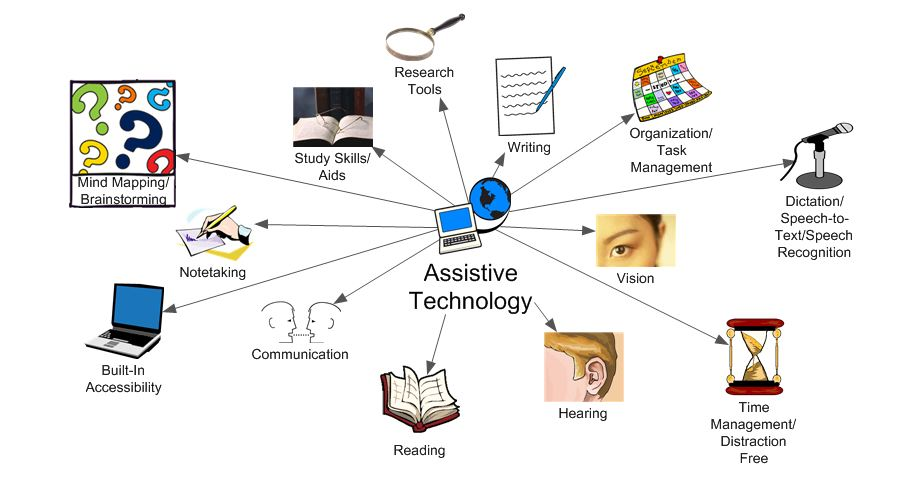
\includegraphics[width=0.8\textwidth]{./Web_accessibility_images/AT-Mind-Map-for-Website.jpg}
   	 \caption{Assistive Technology Mind Map for Web}
	\end{figure}

	\subsection{Screen Readers}

	Screen readers are essential software applications designed to translate digital visual information into synthesized speech or 
	tactile Braille displays. They interact directly with browser accessibility APIs and the Document Object Model (DOM) rather than 
	analyzing the visual layout. Popular implementations include NVDA, JAWS, Apple VoiceOver, and Google TalkBack. 

	Developers support screen readers by implementing native semantic HTML elements (\texttt{<nav>}, \texttt{<main>}, 
	\texttt{<button>}), providing precise image \texttt{alt} text, configuring WAI-ARIA attributes (\texttt{aria-expanded}, 
	\texttt{aria-label}), and defining \texttt{aria-live} regions for dynamic content updates.

	\begin{figure}[h!]
  	  \centering
  	  \includegraphics[width=0.8\textwidth]{./Web_accessibility_images/1*cYOB76MZE6DNDBlwNrsUvQ.jpg}
   	 \caption{Screen Reader User Interaction}
	\end{figure}

	\subsection{Magnifiers}

	Screen magnifiers enlarge visual content on a digital display, assisting individuals with low vision, visual fatigue, or partial sight 	
	impairments. Modern magnification software provides adaptive zoom levels, continuous cursor and focus tracking, customizable 	
	viewport configurations, high-contrast pointer indicators, and dynamic font smoothing.

	Web developers accommodate screen magnifiers by designing flexible, responsive layouts that maintain structure when zoomed
	 up to 400\%. Crucially, layouts must prevent text clipping, overlapping containers, or forced horizontal scrolling at high zoom 
	 levels.

	\begin{figure}[h!]
  	  \centering
   	 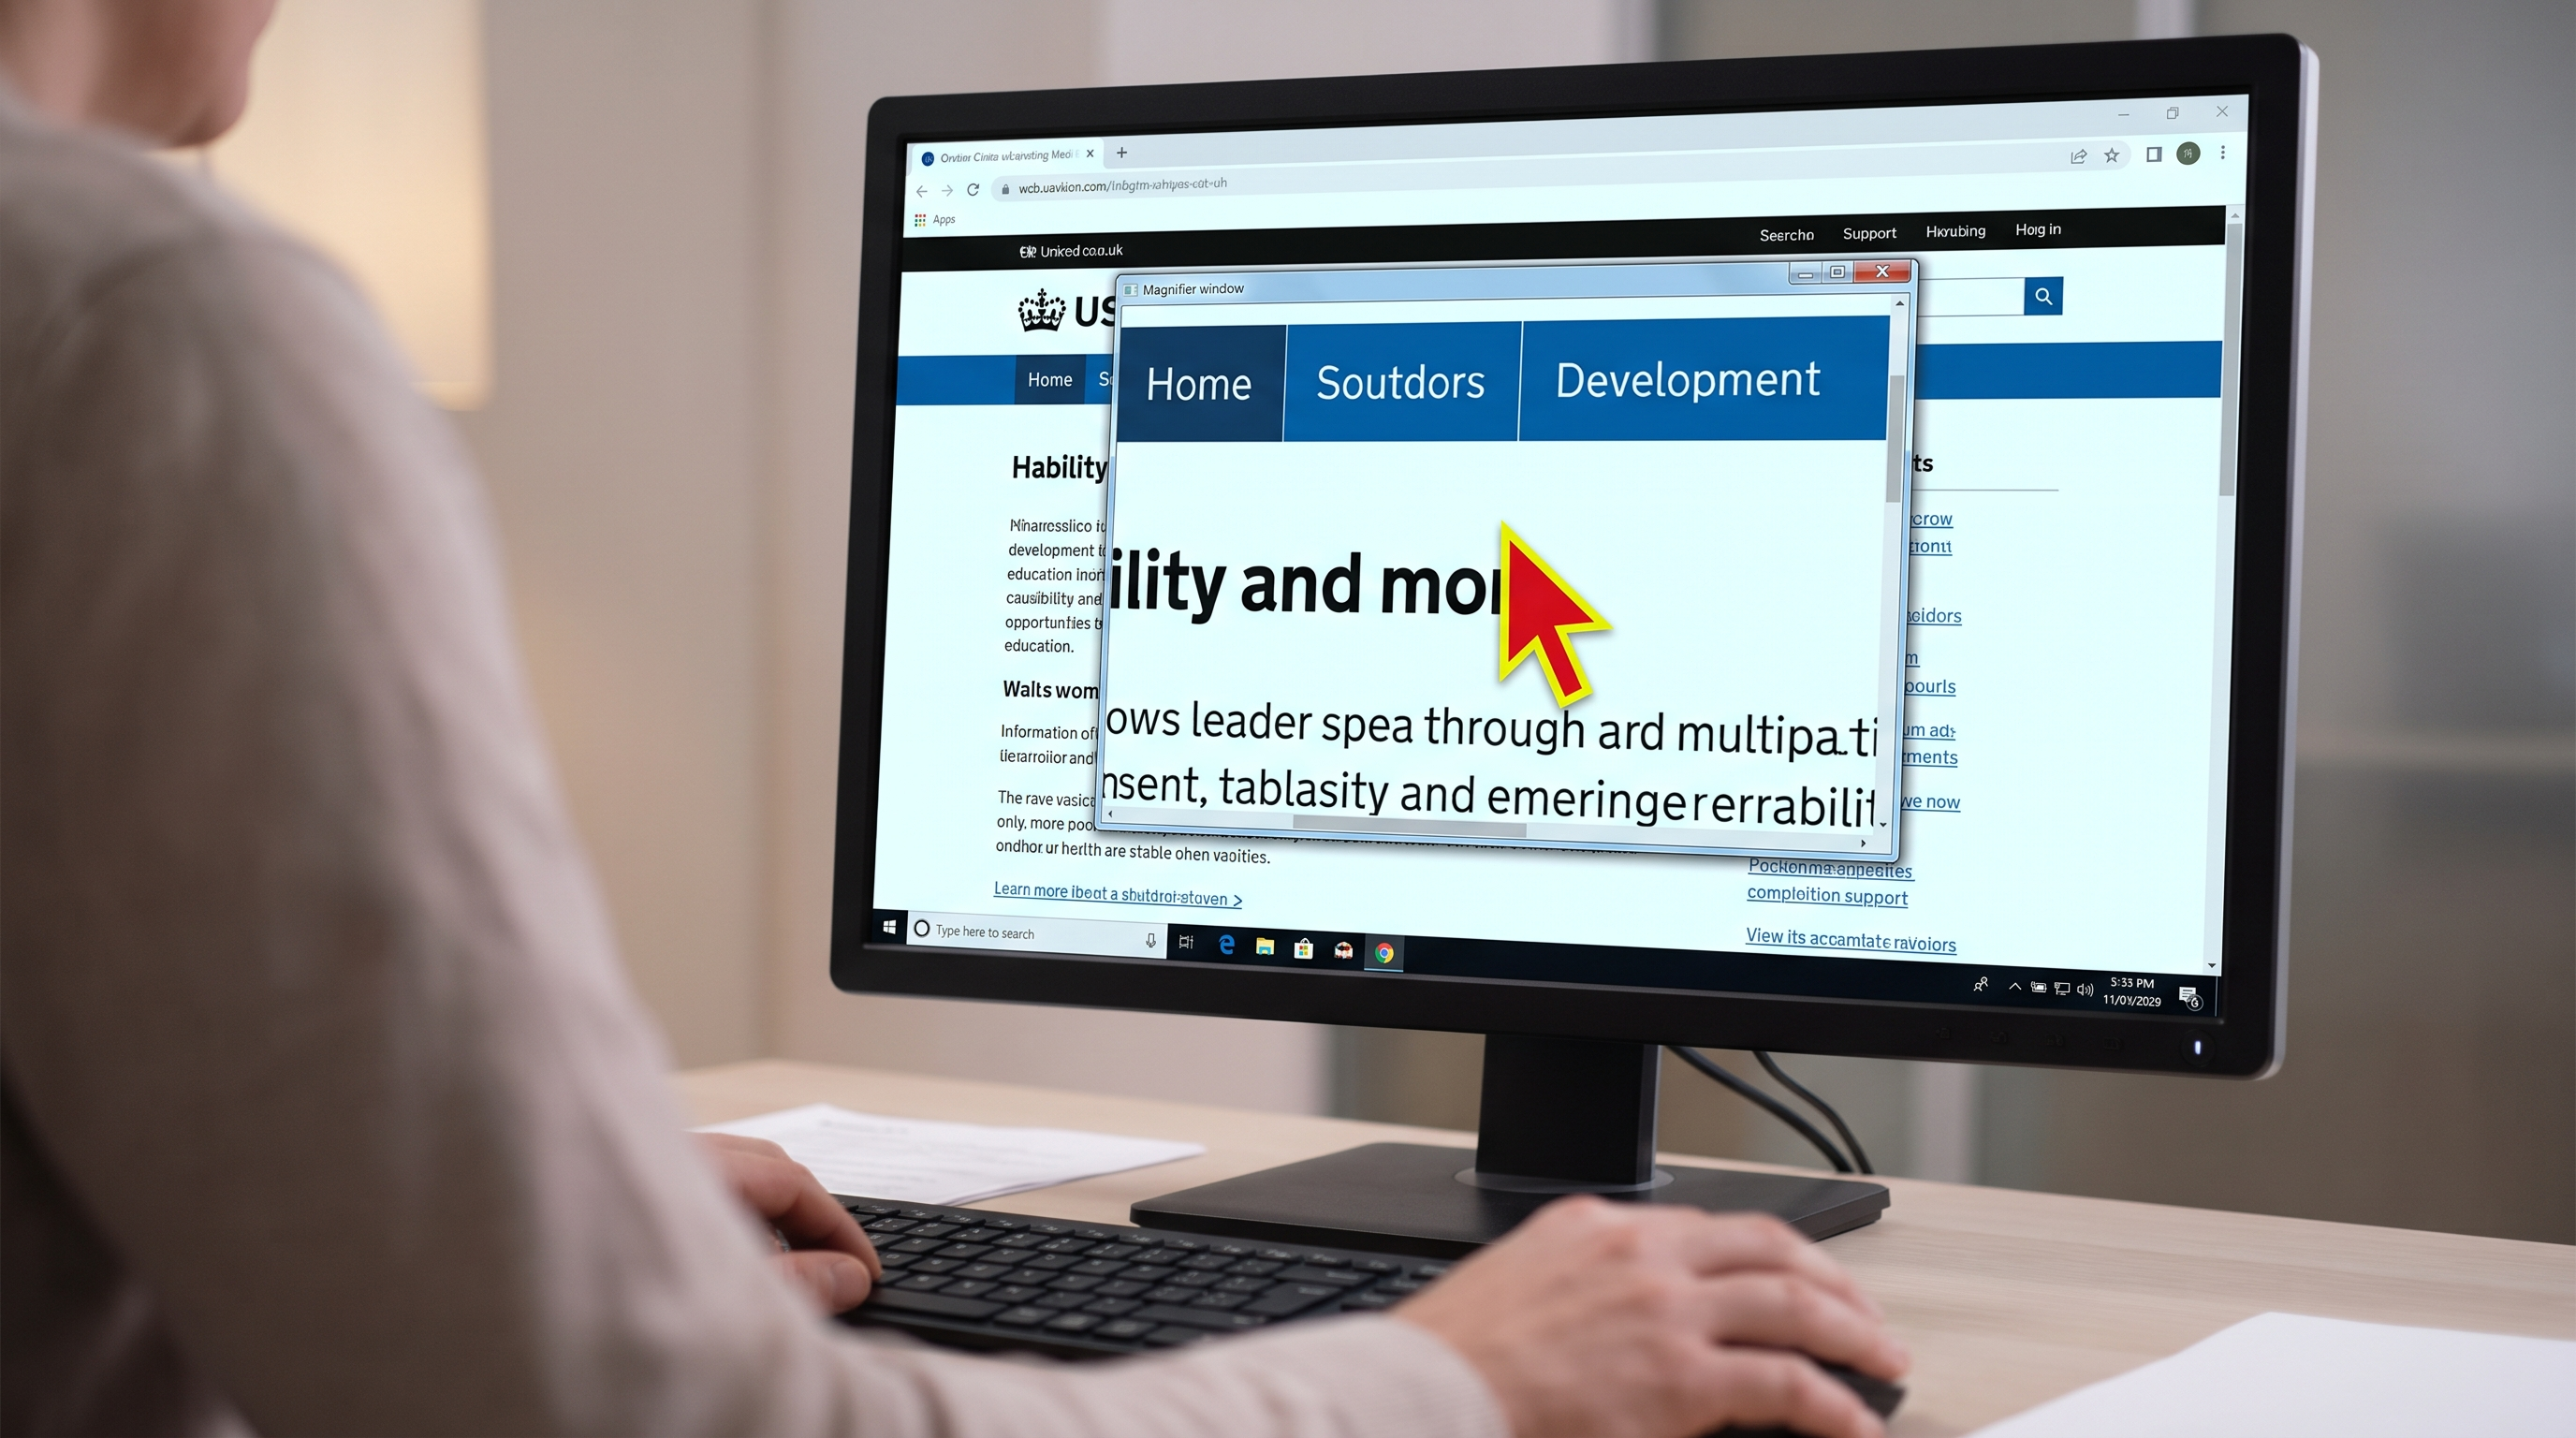
\includegraphics[width=0.8\textwidth]{./Web_accessibility_images/Magnifiers.jpg}
    	\caption{Screen Magnification on a Computer Monitor}
	\end{figure}

	\subsection{Keyboard Navigation}

	Keyboard navigation enables users to browse and interact with digital interfaces entirely without a physical mouse or 
	touchscreen. This access mode is critical for individuals with fine motor control challenges, tremors, or permanent physical 
	disabilities.

	Compliant web interfaces support full keyboard operation using standard keys (\texttt{Tab}, \texttt{Shift+Tab}, \texttt{Enter}, 
	\texttt{Spacebar}, and arrow keys). Key implementation requirements include maintaining a logical DOM tab order, displaying 
	distinct CSS focus rings (\texttt{:focus-visible}), managing focus inside modal dialogs, and providing skip-to-content links.

	\subsection{High Contrast and Custom Color Themes}

	High contrast modes and custom color themes adjust visual presentations for users with color blindness, photophobia, low vision, 
	or sensitivity to visual brightness. Developing accessible visual themes requires meeting standard WCAG contrast ratios (such as
	 a minimum of 4.5:1 for standard body text), integrating operating system color modes (e.g., CSS \texttt{forced-colors}), and 
	 offering user-selectable dark and light themes.

	Furthermore, accessible design dictates that color must never serve as the sole method for conveying information, signaling 
	interactions, or displaying validation errors.

	\begin{figure}[h!]
  	  \centering
  	  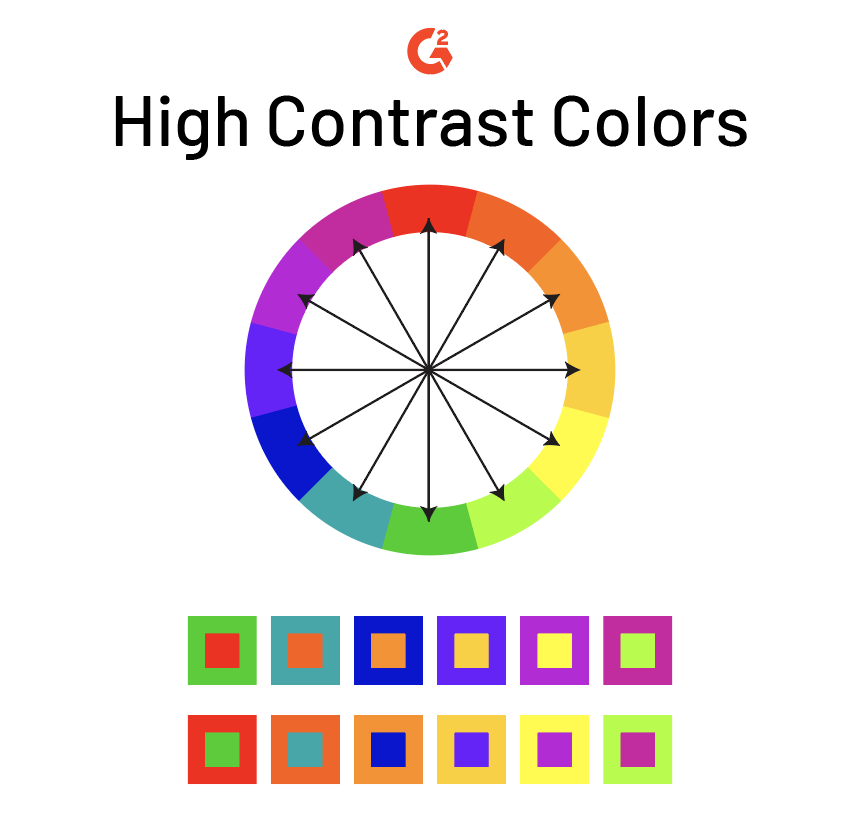
\includegraphics[width=0.4\textwidth]{./Web_accessibility_images/high contrast colors.png}
  	  \caption{High Contrast Color Palette}
	\end{figure}

	\subsection{Alternative Input and Speech Recognition}

	Alternative input methods and speech recognition software enable individuals with severe motor disabilities or limb differences to 	
	interact with web interfaces through voice commands, eye-tracking hardware, head pointers, or single-switch devices. Users can 	
	issue spoken navigation commands or trigger interface actions through switch cycles.

	Designing for alternative input requires large click targets, visible activation labels matching accessible DOM names, avoidance of 	
	complex multi-touch gestures, and robust native form elements.

	\begin{figure}[h!]
   	 \centering
   	 
\includegraphics[width=0.4\textwidth]{./Web_accessibility_images/voicerecog.png}
    	\caption{Voice Recognition and Speech Input}
	\end{figure}

\newpage
%%%%%%%%%%%%%%%%%%%%%%%%%%%%%%%%% Documentation [COMPLETE] ~Coffee

\section{Sources}

	\subsection{links}
	
	\begin{itemize}
	\item  \url{https://www.w3.org/TR/2024/REC-WCAG22-20241212/} 		%WCAG Guidelines and Standards:
	\item 
	  \url{https://books.google.ch/books?hl=it&lr=&id=qaNxEQAAQBAJ&oi=fnd&pg=PP1&dq=Interface,+inclusive+design+principles&ots=N3sSFD2wu6&sig=joiCB_Rtm_UsUrDiABZb9EwNItE&redir_esc=y#v=onepage&q&f=true}	%Inclusive design principles
	   \item  \href{https://www.w3.org/WAI/}{W3C Web Accessibility Initiative}	%W3C WAI Home
   	 \item  \href{https://www.w3.org/WAI/people-use-web/}{W3C: How People with Disabilities Use the Web}	%W3C How People Use the Web
    	\item  \href{https://www.w3.org/WAI/people-use-web/tools-techniques/presentation/}{W3C WAI: Presentation and Customization Tools}	%Tools and Techniques
    	\item  \href{https://webaim.org/}{WebAIM: Web Accessibility in Mind}		%WebAIM Main Resource
    	\item  \href{https://www.w3.org/WAI/perspective-videos/}{W3C Web Accessibility Perspectives Videos}	%W3C Perspectives Overview
	\item https://www.gartner.com/en/newsroom/press-releases/2026-02-26-gartner-says-surging-memory-costs-will-reduce-global-	pc-and-smartphone-shipments-in-2026
	\item https://www.itu.int/en/mediacentre/Pages/PR-2026-11-03-Facts-and-Figures.aspx
	\item https://leadership.ng/smartphones-cost-76-of-monthly-income-in-sub-saharan-africa/\#1
	\item https://www.techspot.com/news/114436-teamgroup-warns-memory-shortage-has-not-reached-peak.html
	\item https://www.w3.org/WAI/business-case/\#is-there-a-business-case-for-accessibility % this should be before the part 4 , also look for the recent href
	\end{itemize}

	\subsection{images}

	\begin{itemize}
    	\item fig.2.1 :  \url {https://blog.adobe.com/en/publish/2018/04/02/different-breaking-accessibility-universality-inclusion-design}
	\item fig.2.2 :  \url{ https://dashdevs.com/blog/inclusive-design-and-ux-accessibility/}
	\item fig.2.3 :  \url{ https://www.singlegrain.com/blog-posts/design/design-principles-for-accessibility/}
	\end{itemize}



\end{document}
